\subsection{Weight Training}

Weight lifting is popular among those training for a particular sport, or as a form of recreation. While training programmes include many exercises, there are three lifts that are considered fundamental and are the basis of the majority of effective routines. These three lifts are the three powerlifting techniques.

Powerlifting is a sport where the objective is to lift the maximum possible weight in each of three movements. These movements are the squat, bench press and deadlift.

In a competition, powerlifters are given three attempts at each of the three lifts, and the weights of the maximum successful lift for each movement are summed to give the lifter's `total'. The total is their score in the competition, and the lifter with the highest score in their weight category is deemed the winner.

Whether training for powerlifting or other sports, the squat, bench press and deadlift are an integral part of training for any gym-goer. These three lifts are detailed below.
\pagebreak
\subsubsection{Squat}

The squat is the first of the three lifts to be performed in a powerlifting competition, and is a movement in which the legs are the main driving force. The barbell is placed on the lifter’s shoulders or upper back, and the lifter must bend at their knees and hip to bring their hip joint below their knees. When they have reached this position, they must then push hard with their legs to return to an upright position. Figure~\ref{fig:squat_stages} shows an example of a squat.

\begin{figure}[H]
    \centering
    \subfigure[Begin]{
            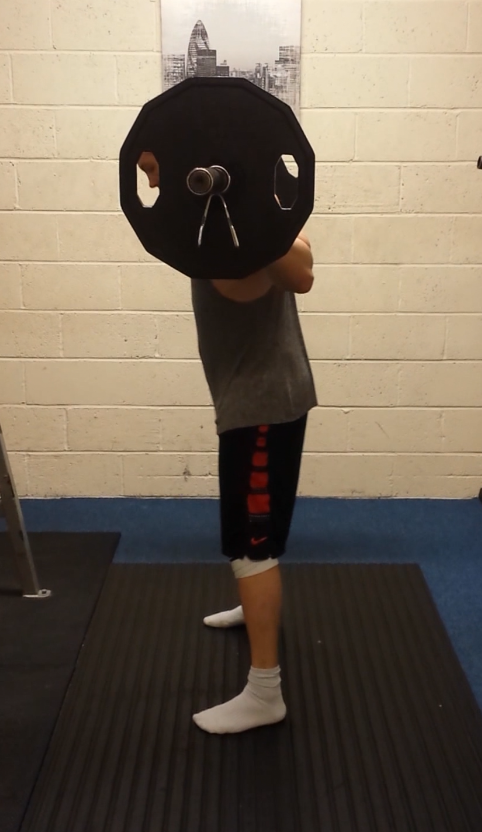
\includegraphics[height= 7cm]{intro/images/squat_start}
    }
    \subfigure[Middle]{
            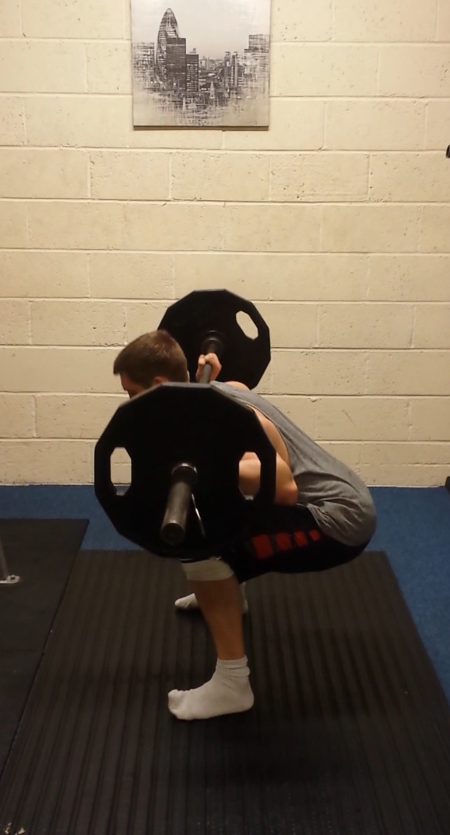
\includegraphics[height= 7cm]{intro/images/squat_middle}
    }
    \subfigure[End]{
            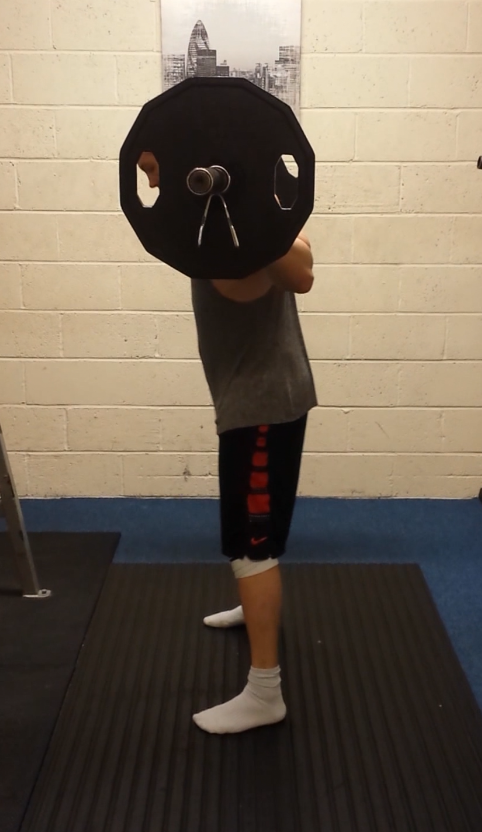
\includegraphics[height= 7cm]{intro/images/squat_start}
    }
\caption{The stages of a squat}
\label{fig:squat_stages}
\end{figure}

The International Powerlifting Federation regulations\cite{ipf} give a list of the criteria used to deem whether a lift is successful or not. In competition, the main objective is to reach sufficient depth and return to the upright position with no external help. In addition, when the lifter has started their ascent, there must be no further downward movement. In training, it is considered good practice for a lifter to keep their shins reasonably perpendicular to the ground in order to minimise the risk of knee injury. It is also advantageous for the lifter to keep the bar directly above their feet at all times during the lift, establishing a better position to drive the bar upwards.
\pagebreak
\subsection{Bench Press}

The bench press is an upper body movement requiring the lifter to lie on a bench parallel to the ground, with the barbell above them on a rack. The lifter must grip the barbell with their hands, removing it from the rack and allowing it to descend onto their chest by bending their elbows and shoulders. When the bar touches the lifter's chest, they must push vertically to lock out their elbows. A bench press is considered successful if the barbell touches the chest and the elbows are successfully locked to full extension upon completion. Figure~\ref{fig:bench_stages} shows an example of a bench press.

\begin{figure}[H]
    \centering
    \subfigure[Begin]{
            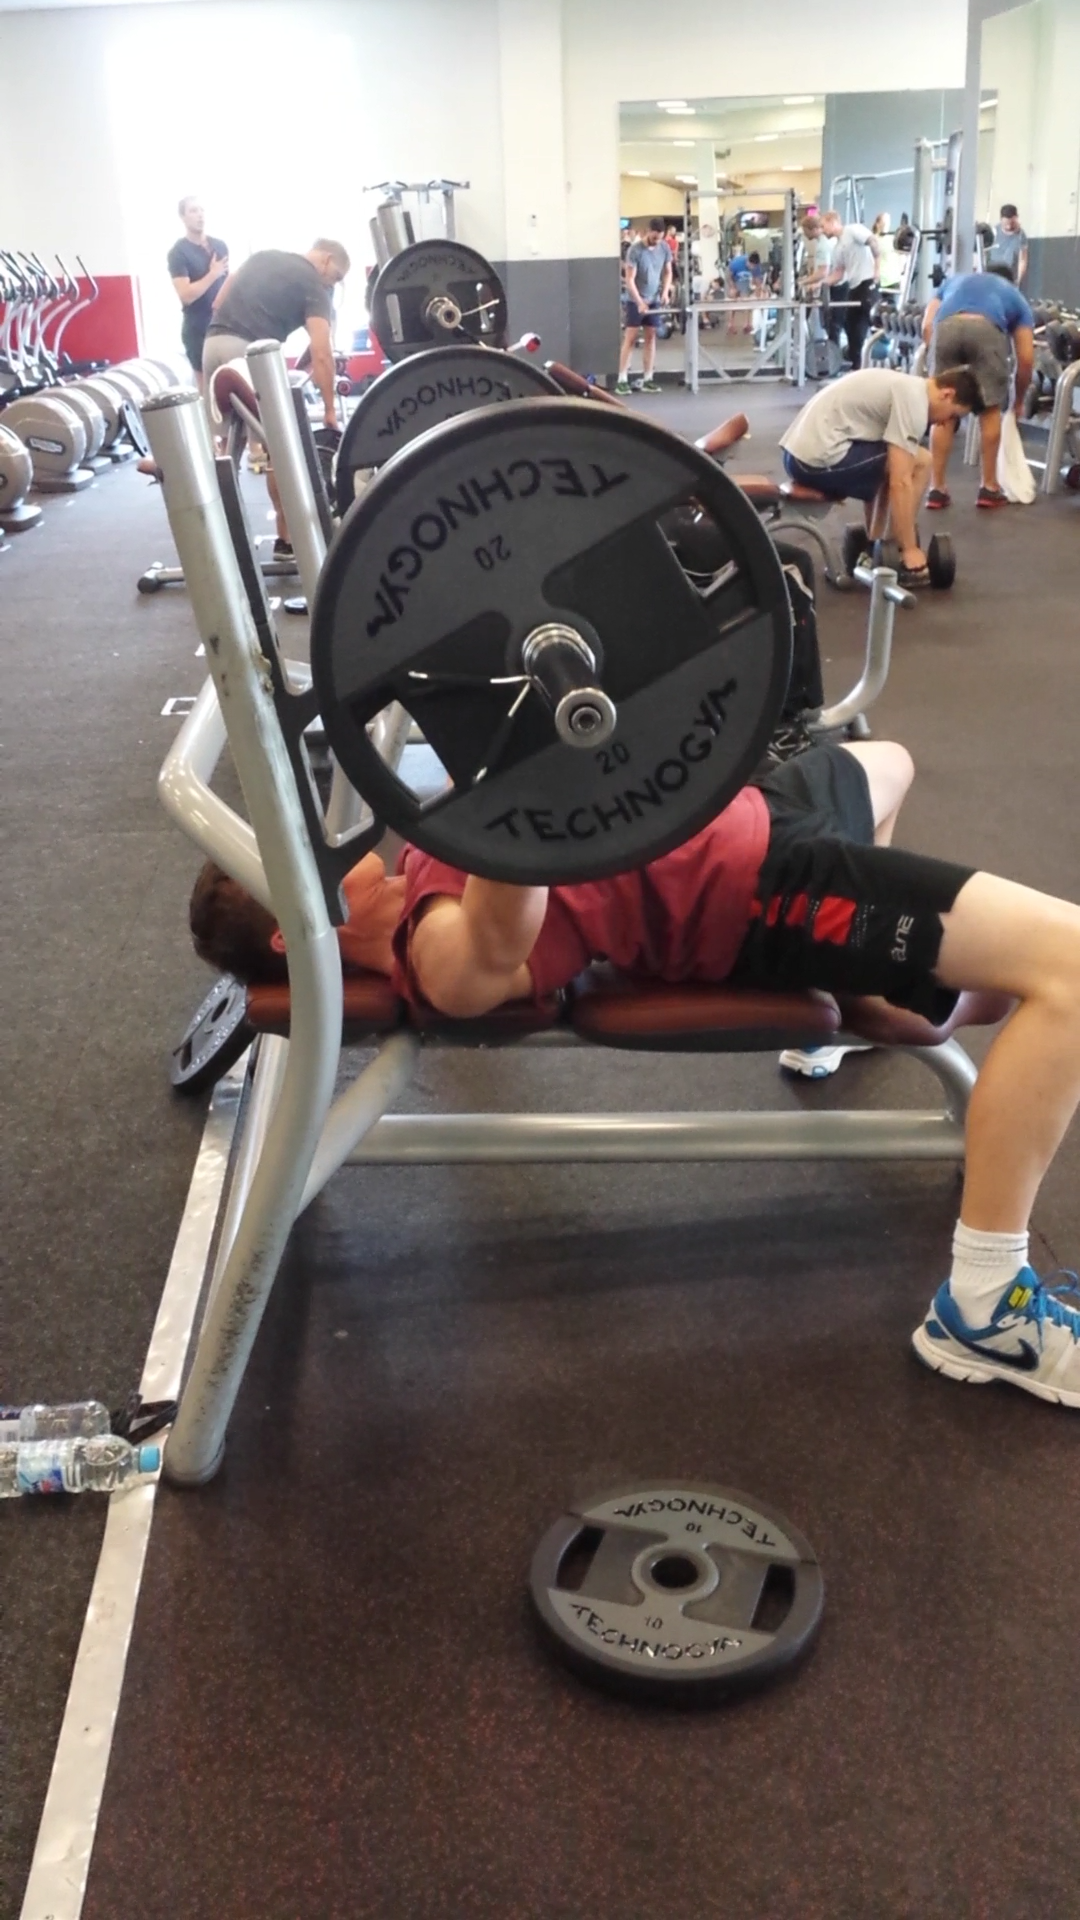
\includegraphics[height=7cm]{intro/images/bench_start}
    }
    \subfigure[Middle]{
            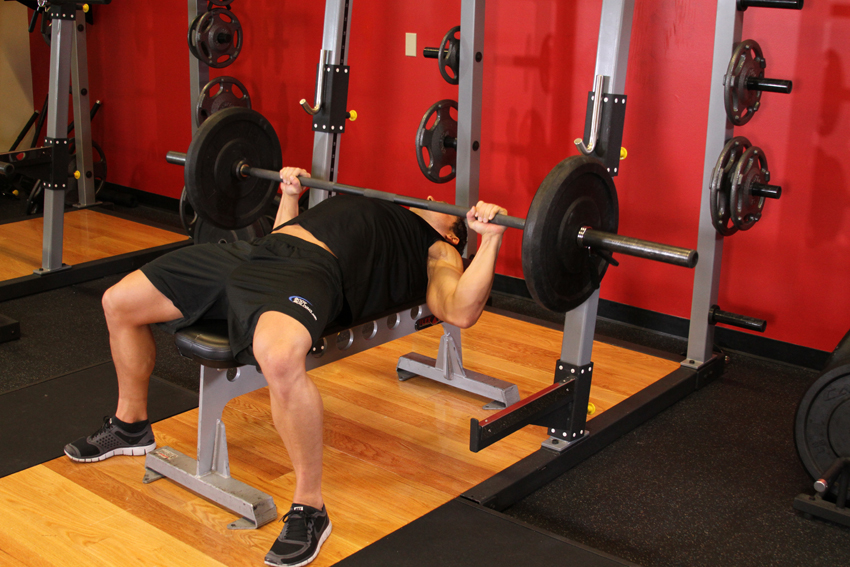
\includegraphics[height=7cm]{intro/images/bench_middle}
    }
    \subfigure[End]{
            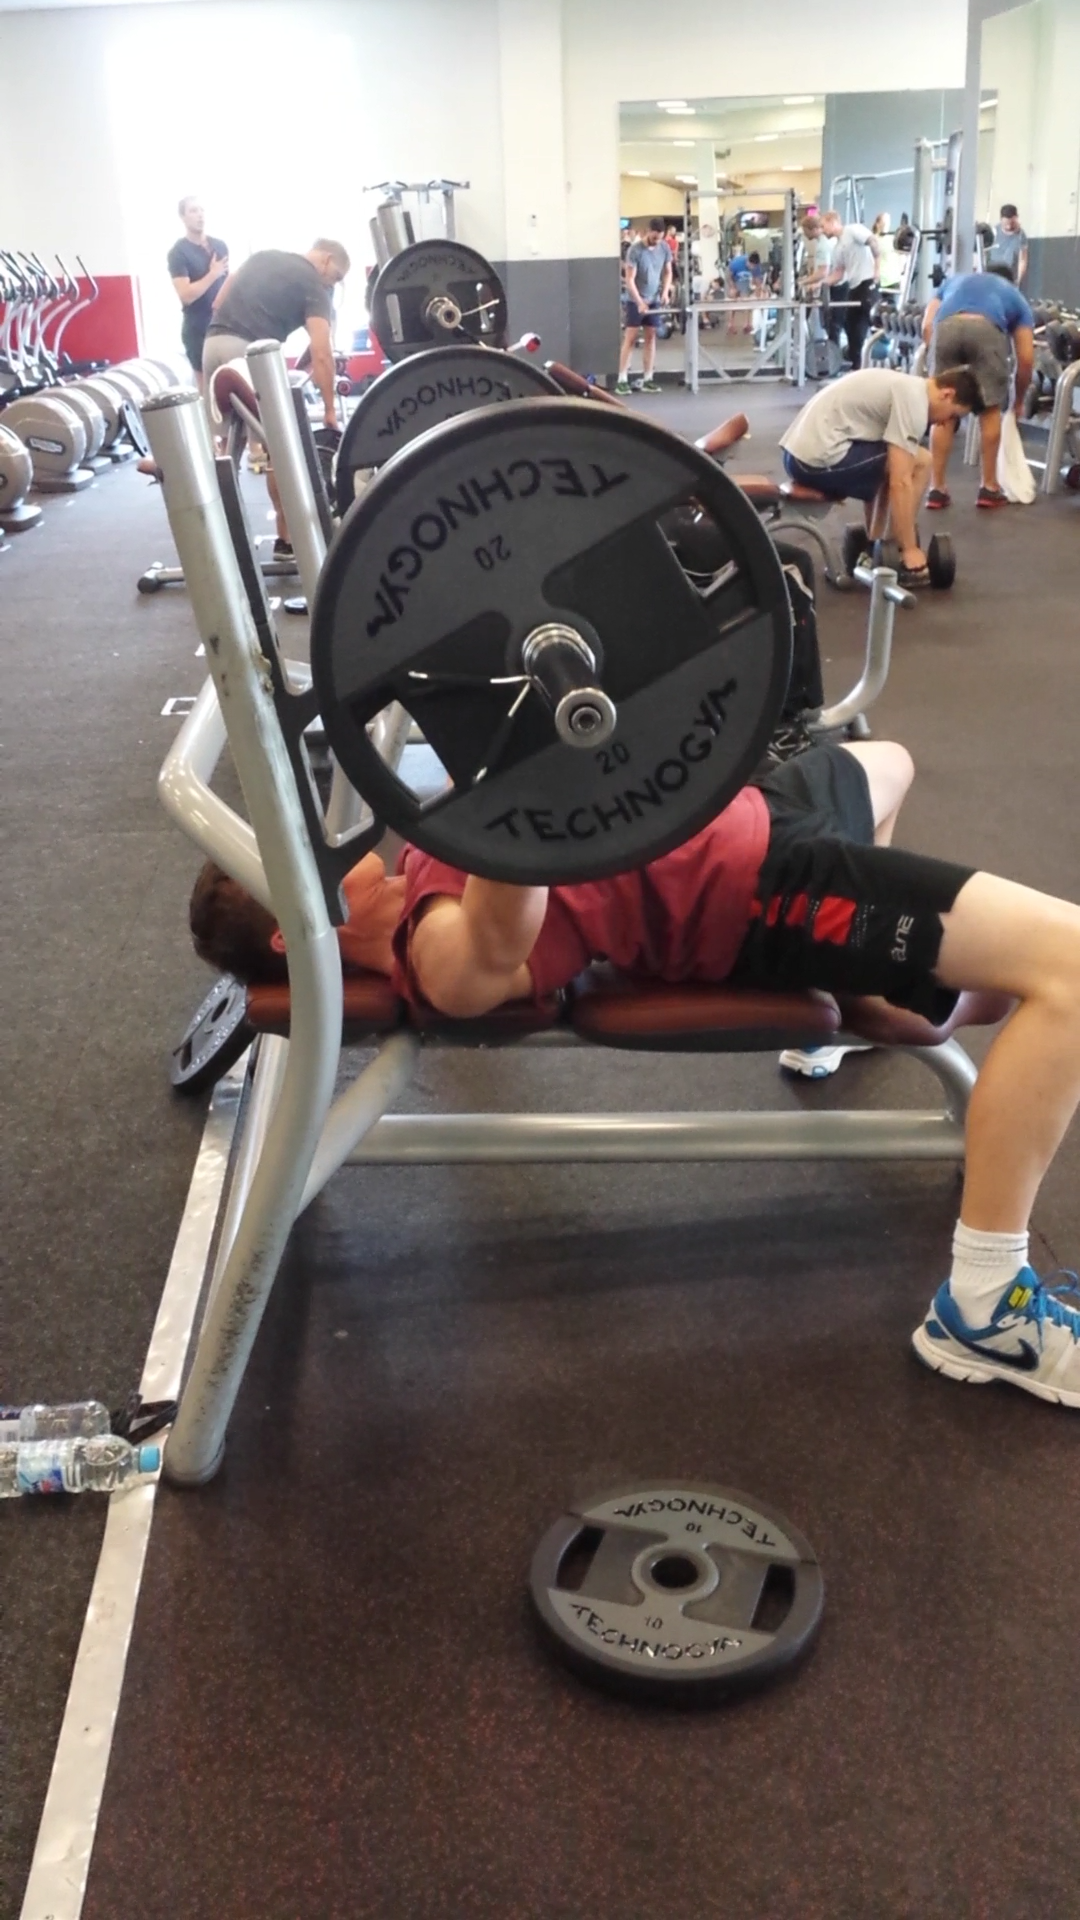
\includegraphics[height=7cm]{intro/images/bench_start}
    }
\caption{The stages of a bench press}
\label{fig:bench_stages}
\end{figure}

The International Powerlifting Federation regulations\cite{ipf} state that during the bench press, the body position of the lifter must not change, ie. the hips, shoulders and head should remain in contact with the bench at all times.
\pagebreak
\subsubsection{Deadlift}

A deadlift is the final exercise performed at a powerlifting competition. In this movement, the barbell starts stationary on the ground. The barbell is gripped in the hands of the lifter, and the lifter must successfully ‘stand up’ whilst holding the weight. A lift is considered complete when the lifter is in a fully upright position, with knees locked and shoulders back. This movement requires activation of the entire posterior chain, that is the use of the muscles on the rear of the legs and back. Figure~\ref{fig:dead_stages} shows an example of a deadlift.

\begin{figure}[H]
    \centering
    \subfigure[Begin]{
            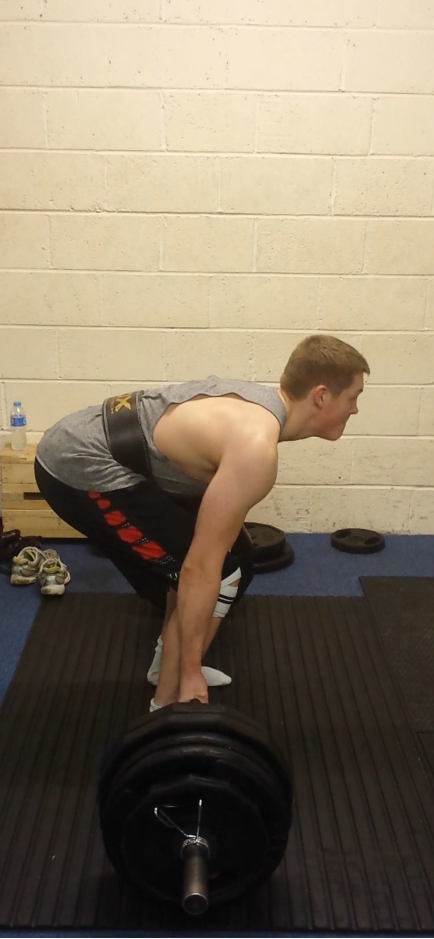
\includegraphics[height= 7cm]{intro/images/dead_start}
    }
    \subfigure[End]{
            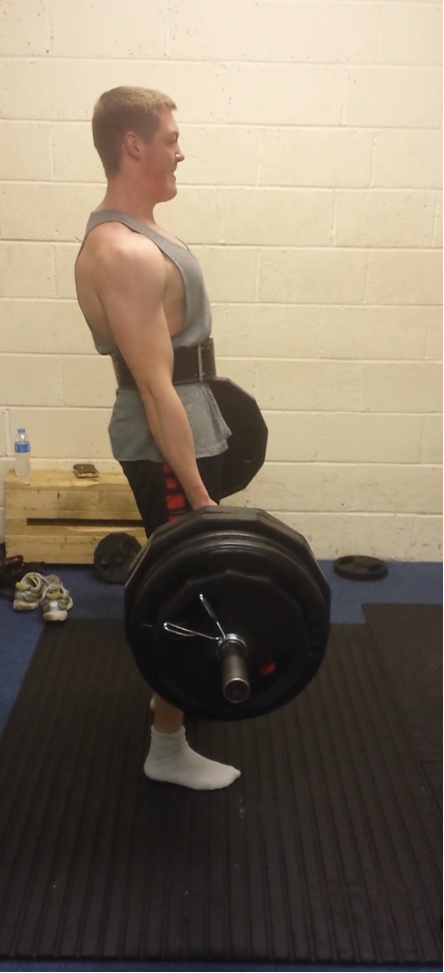
\includegraphics[height= 7cm]{intro/images/dead_end}
    }
\caption{The stages of a deadlift}
\label{fig:dead_stages}
\end{figure}

The International Powerlifting Federation regulations\cite{ipf} state that a deadlift should finish in the upright position, with no downward movement until this point. In training it is considered good practice to ensure that a neutral spine is maintained throughout the lift, that is that there should be no rounding of the back.

